\documentclass[a4paper,12pt,parskip,bibtotoc,liststotoc]{article}
    %Festlegung der Dokumentenklasse, zahlreiche Vereinbarungen über Layout, Gliederungsstrukturen,
    %bsp. article -> section, subsection..., book -> chapter, section...
    %parskip = Abstand zwischen Absätzen, Veränderung durch \setlength

\usepackage[ngerman]{babel}     %Neue deutsche Rechtschreibung, Umlaute können geschrieben werden
\usepackage[utf8]{inputenc}     %direkte Angabe von Umlauten
\usepackage[T1]{fontenc}        %Silbentrennung bei Sonderzeichen
\usepackage{setspace}           %für Zeilenabstand
\usepackage[notindex,nottoc]{tocbibind}   %Inhaltsverzeichnisse erstellen


\usepackage{mathptmx,charter,courier} % Für schöne Schriften
\usepackage[scaled]{helvet}     		%Serifenlose Schrift wird in Helvetica geschrieben
\usepackage{calligra}    				%Calligra Schriftart
\usepackage{eufrak}      				%mathematische Symbole


%zusätzliche benötigte Pakete
\usepackage{graphicx}           %Graphik
\usepackage{amsmath}    		%Mathematik
\usepackage{natbib}             %Zitate
\usepackage{marvosym}           %enthält Symbole wie das Eurozeichen
\usepackage{eurosym}

%\setcounter{secnumdepth}{3}
%\setcounter{tocdepth}{3}



\usepackage{mdwlist}   			%Verringerung Abstand zwischen items -> \begin{itemize*} \end{itemize*}
\usepackage[labelsep=space,justification=centering]{caption} % Abbilungd-/Tabellen Über-/Unterschriften

%\usepackage{hyperref}  		%erlaubt Links innerhalb des pdf-Dokuments zu erzeugen

\setlength{\parindent}{0pt}     %Verhinderung des horizontalen Einrückens zu Beginn eines Absatzes

%Seitenlayout
\topmargin -0.9cm       %Vertikaler Abstand der Kopfzeile von der Bezugslinie
\textheight 25cm        %Abstand der Grundlinie der Kopfzeile zum Haupttext
\textwidth 16.5cm       %Breite des Haupttexts
\footskip 1cm           %Abstand der Grundlinien der letzten Textzeile und der Fußzeile
\voffset -0.5cm         %Vertikale Bezugspunktposition
\hoffset -1.2cm         %Horizontale Bezugspunktposition

\onehalfspacing         %anderthalbzeiliger Abstand

\newcommand{\url}{\;}   %URL im Literaturverzeichnis

%eigene Befehlsdefinitionen
\newcommand{\be}{\begin{equation}}     %Mathematische Umgebung
\newcommand{\ee}{\end{equation}}
\newcommand{\bea}{\begin{eqnarray}}
\newcommand{\eea}{\end{eqnarray}}
\newcommand{\bean}{\begin{eqnarray*}}  %ohne Nummerierung
\newcommand{\eean}{\end{eqnarray*}}    %ohne Nummerierung

%%%%%%%%% ACHTUNG, HIER NEU HINZUGEFÜGTE PACKAGES%%%%%%%%%%%%%%%%%%%%%%%%%%%%
%

\usepackage{titlesec}

\setcounter{secnumdepth}{4}

\titleformat{\paragraph}
{\normalfont\normalsize\bfseries}{\theparagraph}{1em}{}
\titlespacing*{\paragraph}
{0pt}{3.25ex plus 1ex minus .2ex}{1.5ex plus .2ex}

%
%%%%%%%%%%%%%%%%%%%%%%%%%%%%%%%%%%%%%%%%%%%%%%%%%%%%%%
\begin{document}

\pagenumbering{roman}  %römische Seitennummerierung
%%%%%%%%%%%%%%%%%%%%%%%%%%%%%%%%%%%%%%%%%%%%%%%%%%%%%%
%
%    Titelseite
%
%%%%%%%%%%%%%%%%%%%%%%%%%%%%%%%%%%%%%%%%%%%%%%%%%%%%%%
\thispagestyle{empty}  %keine Seitenzahl auf Titelseite
Leibniz Universität Hannover\\
Wirtschaftswissenschaftliche Fakultät\\
Institut für Produktionswirtschaft\\
Prof.\ Dr.\ Stefan Helber

\vspace{5cm}

\begin{center}
Hausarbeit \\
im Rahmen des Seminars zur Produktionswirtschaft im WS 2016/17 \\
(Veranstaltungs-Nr. 171137)

\vspace{2.5cm}

Thema Nr. ..\\[1mm]    %hier Themennummer eintragen
{\Large Titel }
\end{center}

\vspace{7.5cm}

Vorname Name \\
Straße Hausnummer \\
PLZ Ort \\
Matr.-Nr. 1234567 \\[3mm]
Abgabedatum:


\newpage

%Inhaltsverzeichnis erstellen
\tableofcontents

\newpage  %neue Seite

%Abbildungsverzeichnis erstellen
\listoffigures

%Tabellenverzeichnis erstellen
\listoftables

%Abkürzungsverzeichnis
\section*{Abkürzungsverzeichnis}
\addcontentsline{toc}{section}{Abkürzungsverzeichnis}
\begin{table}[h!]
    \vspace*{-3mm}
    \hspace*{2mm}
  \renewcommand{\arraystretch}{1,5}
    \begin{tabular}{ll}  %hier die Spaltenausrichtung und Anzahl eintragen
     LP	        & Linear Programming\\
     MIP		& Mixed Integer Programming\\
     OR		    & Operations Research\\
     RCPSP      & Resource-Constrained Project Scheduling Problem\\
     TSP        & Traveling Salesman Problem\\
     WYSIWYG    & What You See Is What You Get\\
     WYSIWYM    & What You See Is What You Mean\\
	\end{tabular}
\end{table}

%Symbolverzeichnis
\section*{Symbolverzeichnis}
\addcontentsline{toc}{section}{Symbolverzeichnis}
\begin{table}[h!]
    \vspace*{-3mm}
    \hspace*{2mm}
  \renewcommand{\arraystretch}{1,5}
    \begin{tabular}{ll}  %hier die Spaltenausrichtung und Anzahl eintragen
     $\alpha$	& alpha\\     %hier $-Operatoren verwenden, da mathematischer Ausdruck im Text
	\end{tabular}
\end{table}

\newpage

\pagenumbering{arabic}   %ab hier arabische Seitenzahlen beginnend mit 1



\section{Lösung eines ELRP-TW nach Kleinschmidt durch GA}


\subsection{Simultan-sequentielle Herangehensweise}

Neben der Herangehensweise von Kleinschmidt (2017), wie sie in den vorangegangenen Abschnitten durch das GAMS-Modell näher vorgestellt, analysiert und bewertet wurde, gibt es weitere Möglichkeiten, sich der Problemstellung anzunehmen.
Im Folgenden wird eine Methodik untersucht, die zunächst die Standortbestimmung aus einer Menge an bereits vorgegebenen Standorten untersucht, um sie dann simultan Kunden zuzuweisen.
Dabei wird die simultane Bearbeitung verschiedener Probleme, wie sie bereits bei Kleinschmidt gelebt wird, zumindest in diesem Punkt aufrechterhalten.

Sequentiell an diese simultane Bearbeitung angeschlossen wird dann allerdings die Durchführung einer optimierenden Routenplanung, wobei ein genetischer Algorithmus zur Anwendung herangezogen wird.
Bei großen Datenmengen und knappen Rechnerkapazitäten könnte diese Vorgehensweise durchaus von Vorteil sein, da der genetische Algorithmus ein metaheuristisches Verfahren darstellt, welches üblicherweise in relativ kurzer Rechenzeit an eine solide Lösung gelangt.

Bevor sich der Bearbeitung des VRP mittels einem genetischen Algorithmus gewidmet wird, stellt sich die Frage, wie an das Problem der Standortbestimmung herangegangen werden sollte, wobei mehrere potentielle Ansätze existieren.
Im Folgenden wird sich auf die Erstellung eines Algorithmus konzentriert, der die Lösung eines 'Facility Location Problem' herbeiführen soll.
Dieser wird dann in Python implementiert, um es dadurch zu ermöglichen, die Problemstellung in einer angemessenen Arbeitszeit effizient lösen zu können, nachdem die Grundlagen dieses Problems hinreichend erläutert wurden.


\subsubsection{Das Facility Location Problem}

Das Facility Location Problem (FLP) stellt ein Optimierungsproblem zur Standortbestimmung dar. Im Allgemeinen wird dabei aus einer Menge von Standorten S eine Teilmenge F als Versorgungsstandorte ausgewählt (Vgl. Mahdian et.al,S.1).
Ziel ist es, dass jeder Kunde unter Einhaltung der Zielfunktion (Minimierung der Gesamtkosten) von den verfügbaren Angebotsstandorten versorgt wird.
Dabei ist es durchaus möglich, dass ein Kunde von mehr als einem Standort versorgt wird, sodass dessen Nachfrage bei nachfolgender Betrachtung des VRP von mehreren Touren bedient werden kann.
Nicht nur für die Standortbestimmung von Depots wird das Facility Location Problem angewendet, sondern auch für die Bestimmung der Standorte von Krankenhäusern, Supermärkten oder der Positionierung von Servern (Vgl. Kling ,S.2).

Abbildung 1 stellt zwei mögliche Lösungen eines einfachen FLP dar (Vgl. Kling ,S.2):

\begin{figure}[h!]
  \begin{center}
    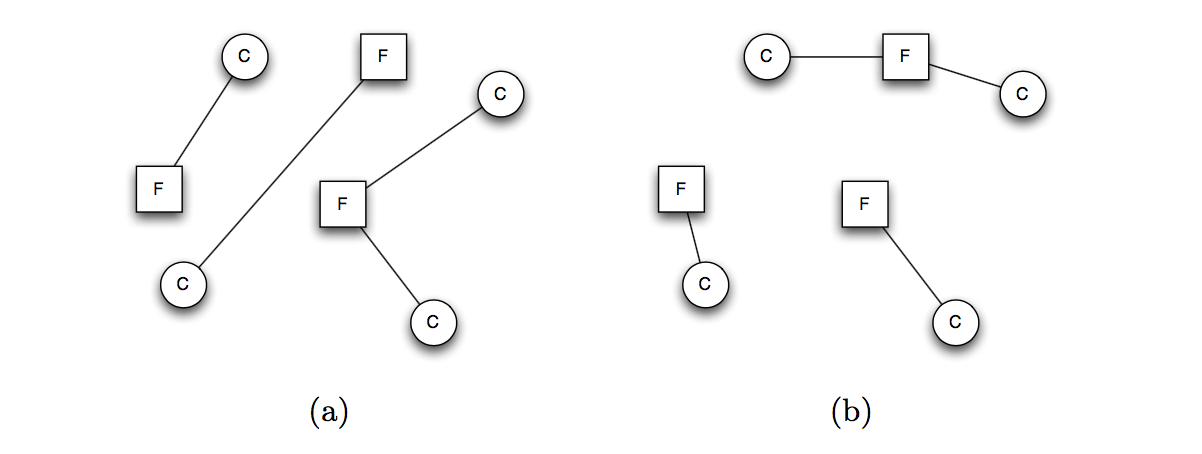
\includegraphics[width=150mm]{FLP}
    \caption{Lösung eines einfachen FLP}  \label{Typen}
    {\footnotesize \textbf{Quelle:} Kling, S.2 }
  \end{center}
\end{figure}


Die beiden Beispiele besitzen jeweils drei Facilities (Depots) und vier Kunden (Nachfrageorte), wobei hier jeder Kunde nur von jeweils einer Basisstation beliefert wird, auch wenn andere Szenarien denkbar sind.
Wählt man nun die euklidischen Distanzen zwischen den Knotenpunkten als einzigen Kostenfaktor, ist es offensichtlich, dass Lösung b effizienter ist als a, da die Distanzen zwischen Depot und Kunden insgesamt geringer sind. 
Man spricht in diesem Fall von Verbindungskosten, wobei es allerdings ungenügend ist, sich nur auf die Verbindungskosten zu fokussieren, da in der Realität meistens noch Betriebskosten für Depots anfallen.
Zu diesen Betriebskosten zählen neben fixen Kosten, wie sie bei der Eröffnung einer neuen Basisstation entstehen würden, auch variable Kosten in Form von Personalkosten, die sich wiederum an den Öffnungszeiten der jeweiligen Basisstationen orientieren.

Wie bereits erwähnt ist F die Menge der Versorgungseinrichtungen (Facilities), in diesem Fall also die Menge aller Depots. 
Mit dem Parameter C werden im Folgenden die Anzahl aller Kunden beschrieben. 
Des Weiteren besitzen die Depots nicht-negative Kostenfunktionen f, welche die Betriebskosten (fix und variabel) jedes Depots darstellen. 
Eine Lösung ist gegeben durch eine Auswahl von $I \subset  F$ Depots, die in Betrieb genommen werden sollen sowie einer Zuteilung von $\theta$ der Kunden C zu den Depots I ( Vgl.Kling S.6).
Dementsprechend wird eine Lösung gesucht, in der die Kosten minimiert werden.\\

In dem Fall wird ein Tupel ($\theta$,I) gesucht, welches die Zielfunktion:

\begin{center}
Min $\Sigma f_{i}  + \Sigma c_{i,j}$ (Vgl.Kling S.6)
\end{center}
 
minimiert.
Zusätzlich werden dem Problem die Binärvariablen $x_{i,j}$ und $y_{j}$ hinzugefügt, die den Wert 0 oder 1 annehmen können. Ist $x_{i,j}$ = 1, so wird dem Kunden j ein Depot i zugeordnet. 
Die Variable  $y_{j}$ entscheidet darüber ob ein Depot ausgewählt wird ($y_{j}$ = 1) oder nicht ($y_{j}$ = 0). 
Nachdem fixe Kosten $f_{i}$ durch variable Kosten ersetzt werden und die Kosten der Lieferwege durch einen einheitlichen Satz c ersetzt werden, um die Kostenfunktion zu Vergleichszwecken der aus dem GAMS-Modell anzupassen, entsteht dadurch eine modifizierte Zielfunktion, welche auch in den nachfolgenden Kapiteln Anwendung findet:


\begin{center}
Min $\Sigma_{j} (close_{j}-open_{j})\cdot cp \cdot y_{j}  + \Sigma_{i}\Sigma_{j} d_{i}*x_{i,j} \cdot c$
\end{center}

Unter den Nebenbedingungen:

\begin{equation} \label{eq:test}
$d_{i,j}\cdot \beta_{i,j} <= M_{j}\cdot y_{j}$
\end{equation}

\begin{equation} \label{eq:test}
$x_{i,j} \in {0,1}$
\end{equation}

\begin{equation} \label{eq:test}
$y_{j} \in {0,1}$
\end{equation}


Die variablen Kosten einer Basisstationseröffnung in Form von Personalkosten finden sich im ersten Term wieder, bei der die konkrete Zeit, die eine Basisstation geöffnet hat, minutenweise mit dem Minutensatz der Personalkosten verrechnet werden.
In den Nebenbedingungen wird zudem aufgezeigt, dass die Kapazität einer Basisstation nicht überstrapaziert werden darf, so wie dies im GAMS-Modell in Restriktion (10) durch die Ungleichung festgehalten wird.
Allerdings ist es im FLP möglich, Kunden mehrmals anzufahren und somit deren Nachfrage auf mehrere Touren aufzuteilen, was nicht den Bedingungen in dem von Kleinschmidt aufgestellten Modell entspricht und zu Vergleichszwecken mit dem obigen GAMS-Modell an Überarbeitung bedarf.

Beim FLP handelt es sich um ein NP-Schweres Problem. 
Solche komplexen Optimierungsprobleme werden meist mit approximativen Algorithmen berechnet.
Durch das FLP gelingt es demnach, eine Teilmenge aus verfügbaren Depots zu ermitteln, die optimal wäre für das in dieser Arbeit vorliegende Problem. 

 


\subsubsection{Modifizierung des Algorithmus zur Lösung des FLP}


Es stellte sich heraus, dass sich das FLP als eine geeignete Problemstellung erweist, dessen Lösungsalgorithmus sich auch in dieser Arbeit als nützlich erweisen könnte, da er bei der Bestimmung optimaler Standorte bereits vorgegebene Standorte untersucht und keine zufällig ausgewählt werden, wie dies bspw. bei üblichen Clusterverfahren der Fall ist.

Das Facility Location Problem ist üblicherweise darauf ausgerichtet, einzelne Kunden mit mehreren Standorten zu beliefern, wobei dies wie bereits beim GAMS-Modell auf lediglich eine Basisstation pro Kunde beschränkt wird.
Die Modifizierung des Algorithmus gelingt, indem der gemischt-ganzzahligen Modellformulierung eine binäre Variable $\beta_{i,j}$ hinzugefügt wird, die die folgende Restriktion erfüllt:

\begin{center}

$\Sigma_{j} \beta_{i,j} = 1$ für alle i

\end{center}

Die der gemischt-ganzzahligen Modellformulierung hinzugefügte binäre Variable \beta_{i,j} bzw. deren Restriktion ist somit vergleichbar mit der Restriktion (9) aus dem GAMS-Modell.

Würde die Modizierung des Algorithmus mit der Implementierung von \beta_{i,j} außen vor gelassen werden, so würde dies im weiteren Verlauf bei der Tourenbestimmung durch den genetischen Algorithmus auch Berücksichtigung finden müssen, was zu einem erheblichen Aufwand führen könnte, sodass diese Erweiterung nachfolgend in einem gesonderten Abschnitt untersucht wird.
Besonders herausfordernd dabei könnte die zusätzlich zu übermittelnden Informationen sein, die aus der Lösung des FLP in den genetischen Algorithmus hineingegeben werden müssen.
Bevor jedoch die Informationen aus der Lösung des FLP in den Ablauf der Lösung des VRP mit einfließen, wird Letzteres zunächst anhand eines Beispiels mit lediglich einer Basisstation im nächsten Kapitel vorgestellt, um diesen dann in den darauf folgenden Kapiteln zu modifizieren.


\subsection{Lösung eines ERP-TW durch GA}

\subsubsection{Grundlagen zum genetischen Algorithmus}

Genetische Algorithmen wurden in Anlehnung an die von Charles Darwin beschriebene natürliche Selektion entwickelt. Es handelt sich um einen biologischen Mechanismus, mit der nach dem Motto „survival of the fittest“ aus einer alten Population eine neue Population entsteht (Vgl. Masum S.126).
Der genetische Algorithmus gehört zu den methaheuristischen Algorithmen und bietet vor allem bei komplexen kombinatorischen Optimierungsproblemen (NP-hard) wie dem Job Shop Scheduling Problem oder dem Vehicle Routing Problem erfolgsversprechende Lösungen an. 
Dabei beschreibt der GA einen evolutionären Prozess, anhand dessen eine neue Population entsteht.
Um den evolutionären Prozess des Algorithmus starten zu können, benötigt man zunächst eine Anfangspopulation. 
Eine Population besteht aus Individuen, die auch als Chromosom bezeichnet werden und jeder für sich eine Lösung der Problemstellung darstellt.
Ist der evolutionäre Prozess abgeschlossen, wird anhand der genetischen Fitness für jedes der Individuen entschieden, ob es in die neue Generation aufgenommen oder eliminiert wird. 
Die Fitness wird meist anhand einer Fitnessfunktion berechnet und variiert von der zu lösenden Problemstellung.
Der evolutionäre Prozess setzt sich im Allgemeinen aus den genetischen Operatoren Selektion, Crossover und Mutation zusammen (Vgl. Masum S.126).
 
Der Crossover bezeichnet einen Vorgang, in dem zwei Elternpaare der Anfangspopulation miteinander gekreuzt werden. 
Die Gene im Chromosom der Elternteile werden dabei systematisch neu zusammengesetzt und bilden ein neues Nachkommen für die nächste Generation (Vgl. Büning et.al S.11).


\begin{figure}[h!]
  \begin{center}
    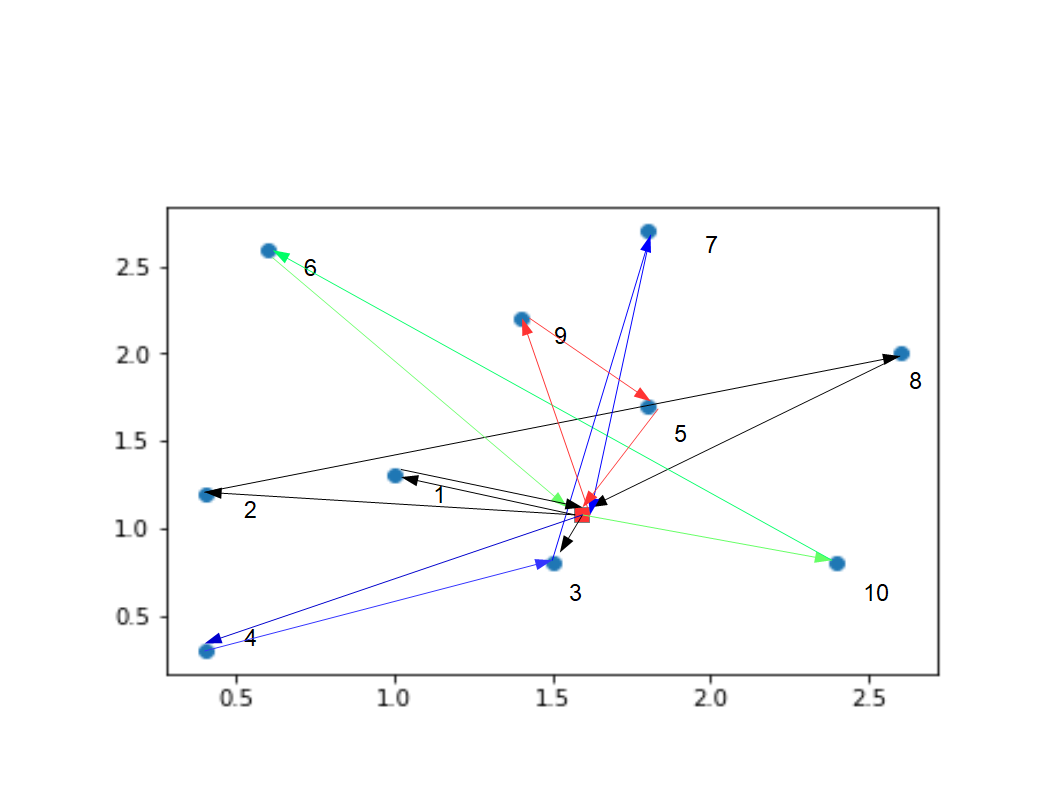
\includegraphics[width=150mm]{vrppp2.png}
    \caption{ Crossover zweier Elternchromosome }  \label{Typen}
    {\footnotesize \textbf{Quelle:} Büning et al., S.11}
  \end{center}
\end{figure}



In der Abbildung x ist ein solcher Crossover-Prozess abgebildet, wobei vielerlei verschiedene Prozesse existieren. 
Die Elternchromosomen sind links dargestellt und die neuen Nachkommen sind auf der rechten Seite zu sehen. 
In diesem Beispiel bestehen die Elternchromosomen aus 8 Genen, von denen jeweils 4 Gene aus einem Elternchromosomen miteinander gekreuzt, bzw. rekombiniert. 
Somit entstehen bei einer Kreuzung zwei neue Nachkommen, jeweils als komplettes Chromosom für die nächste Generation. 
In der Regel wird der Crossover-Prozess für zwei Elternchromosomen jeweils zweimal durchgeführt, sodass die neue Population von $n$ auf $2\cdot n$ Individuen verdoppelt wird.

Die Kreuzung selbst kann durch eine Crossover-Wahrscheinlichkeit gesteuert werden. 
Bei einer Crossver-Wahrscheinlichkeit von 60\% werden bspw. durchschnittlich nur 6 von 10 aller Chromosomen miteinander gekreuzt, wobei in der Praxis eine Wahrscheinlichkeit von mehr als 60\% als sinnvoll erwiesen ist, um möglichst viele neue Individuen entstehen zu lassen (Vgl. Büning et. Al, S.11) und so möglicherweise schneller konvergieren zu können.
Ist der Crossover-Prozess abgeschlossen, folgt die Mutation im genetischen Algorithmus.

Im Mutationprozess kommt es zu einer zufälligen Veränderung innerhalb eines Individuums (Chromosom). 
Dabei werden einzelne Gene innerhalb des Chromosoms vertauscht, wobei auch eine deterministisch festgelegte Mutations-Wahrscheinlichkeit eingehalten wird, sodass nicht jedes Chromosom mutiert wird. 
In der Regel wird dabei eine Wahrscheinlichkeit kleiner als 10\% gewählt (Vgl. Büning et.al S.15).
Mit der Mutation wird versucht, die Population zu diversifizieren und neue Individuen, die weder durch den Crossover hervorgebracht wurden noch in der Anfangspopulation vorhanden waren, entstehen zu lassen. Vor allem bei größeren Populationen ist die Mutation durchaus sinnvoll, um Artenvielfalt zu gewährleisten. Sollte man nur den Crossover durchführen, läuft man stets Gefahr, bei einem lokalen Maximum hängen zu bleiben. Durch die Mutation besteht dann die Möglichkeit, von einem lokalen Maximum auf ein globales Maximum zu kommen (vgl. Goncalves et.al, S.82).\\

Nachdem der Crossover und die Mutation beendet worden sind, erfolgt die Selektion der Individuen in die nächste Generation. 
Dabei ist es üblich, dass die besten Chromosome aus den ursprünglichen bzw. neu gebildeten Chromosomen in die neue Generation gelangen, wobei der Rest eliminiert wird. 
Es gibt jedoch verschiedene Verfahren bei der Auswahl der neuen Generation.
Im genetischen Algorithmus nach Goncalves gelangen bspw. alle neu gezeugten Individuen in die neue Generation ohne Rücksicht auf deren Fitness.

Des Weiteren kann die Auswahl der Individuen zufällig anhand einer Glücksrad-Strategie durchgeführt werden, wie sie im genetischen Algorithmus nach Berger und Barkaoui angewendet wird (Vgl. Berger und Barkaoui, S.x).
Dabei wird in einer Art und Weise vorgegangen, dass die neu erzeugten Individuen mit einer bestimmen Wahrscheinlichkeit proportional zu ihrer Fitness selektiert werden (Berger et.al S. 649).


\paragraph{Darstellung der Chromosome}

Ein Chromosom setzt sich aus k Genen zusammen und wird in Vektorform repräsentiert. 
Die konkrete Ausprägung bzw. der Wert eines Gens wird dabei als Allel bezeichnet.
Dabei variiert die Bedeutung der Gene in den unterschiedlichen Problemstellungen. 
Im Job Shop Scheduling Problem können die Gene im Chromosom die Prioritäten und Verspätungszeiten von einzelnen Arbeitsschritten abbilden (vgl. Goncalves et.al, S.82), jedoch auch lediglich den Schedule.
In Bezug auf das Vehicle Routing Problem stellen die einzelnen k Gene die zu beliefernden Kunden dar. 
Damit stellt ein gesamtes Chromosom eine mögliche Route eines Lieferroboters des VRP dar, wobei der Lieferroboter die Kunden in der Reihenfolge abfährt, wie es das Chromosom ihm vorschreibt. 


\subsubsection{Implementierung in Python}

Im Folgenden wird ein einfaches ERP-TW in Python implementiert, wobei es sich dabei um eine Lösung handelt, die auf einem genetischen Algorithmus basiert. 
Die Instanzen, die die Ausgangslage beschreiben, beinhalten dabei Information bezüglich geografischer Daten der Kunden und der einzelnen Basisstation sowie die gesamte Anzahl an Kunden, die von dieser einen Basisstation aus beliefert werden sollen.
Der Algorithmus ist zunächst sehr einfach gehalten, um den Hauptfokus auf die Erläuterung des genetischen Algorithmus zu legen. 
Im weiteren Verlauf dieser Arbeit wird dieser Algorithmus weiter modifiziert und stetig dem GAMS-Modell aus den vorherigen Abschnitten angepasst.

So analysiert der folgende Algorithmus im Gegensatz zu dem von Kleinschmidt (2017) die Ausgangslage mit lediglich einer einzigen Basisstation, von der aus die Fahrzeuge ihre Fahrt zu den einzelnen Kunden aufnehmen und zu der diese im Anschluss auch wieder zurückfahren, sodass die Standortbestimmung innerhalb des Algorithmus wegfällt.
Die maximale Kapazität der Basisstation ist zunächst unbeschränkt und stellt somit keinen eigenen Parameter dar, sodass Restriktion () aus dem GAMS-Modell entfällt. 
Auf zusätzliche Standortbestimmungen mittels Algorithmen zur Lösung des FLP wurde in dieser Arbeit bereits eingegangen, sodass der genetische Algorithmus im weiteren Verlauf so konzipiert werden muss, dass er die Informationen, die es aus der Lösung des FLP erhält, weiterverarbeiten kann.

Die Kapazitäten eines Akkumulators, sowohl hinsichtlich seiner Reichweite als auch seiner zeitliche Reichweite, werden berücksichtigt und können als Parameter selbst bestimmt werden (Restriktion 11, 12), sodass aus dem Modell wie zuvor im GAMS-Modell ein 'Electric Routing Problem with Time Windows' (ERP-TW) entsteht.\\

Ein Unterschied besteht auch in der Handhabung der Zeitfenster:

Werden diese im vorherigen Verfahren noch strikt eingehalten, können sie im Folgenden unter- bzw. überschritten werden, was allerdings zu Warte- bzw. Verspätungskosten führt und sich negativ auf die Fitnessfunktion auswirkt, je nach Gewichtung.
Dies dient lediglich der Vereinfachung des Problems, da sich im Folgenden gänzlich auf den genetischen Algorithmus und dessen Funktionsweise konzentriert werden soll. 
Feinheiten, die zu vergleichbaren Bedingungen führen, wie sie im GAMS-Modell vorliegen, werden in den nächsten Kapiteln vorgenommen. 

Die Geschwindigkeit des Fahrzeugs wird ebenfalls nicht als extra Parameter angegeben, sodass auch die Beachtung der Höchstgeschwindigkeit irrelevant wird.
Im Folgenden wird dabei eine Distanzeinheit in exakt einer Zeiteinheit zurückgelegt, wodurch diese beiden Größen als gleichwertig anzusehen sind und in der kostenminimierenden Zielfunktion als auch eine Größe angesehen werden.
Die Personalkosten wurden nicht berücksichtigt, da lediglich eine Basisstation in Vollzeit geöffnet hat und somit diese bei allen möglichen Lösungen gleich wären, wohingegen Mietkosten für jeden verwendeten Lieferroboter erhoben werden, da es umso effizienter ist, so wenig wie möglich Lieferroboter zu verwenden.
Diese Mietkosten orientieren sich dabei am Parameter $flat$ des GAMS-Modells.

Begonnen wird mit der Ausrichtung aller vorhandenen Lieferroboter an den Koordinaten des Depots, welches den Startort für jegliche Lieferroboter darstellt.
In der Instanz wird das Depot als Kunde 0 dargestellt, um dem Algorithmus nicht zusätzliche Schwierigkeiten beim Einlesen der Informationen zu bereiten.
In einer Matrix werden jegliche Distanzen aller Kunden untereinander abgebildet, wobei sich diese Matrix an eben jener orientiert, die bereits in den Vorkapiteln in GAMS als Parameter verwendet wurde.
Jeder Kunde verfügt außerdem über Informationen bezüglich dem frühesten bzw. dem spätesten Zeitpunkt, in der er beliefert werden kann.
Diese beiden Informationen besitzt auch das Depot, wobei die Informationen hierbei dementsprechend aussagen, wann das Depot öffnet bzw. schließt.
Letztendlich enthält jeder Kunde eine weitere Angabe über die bei ihm vor Ort benötigte Servicezeit.

Zur Veranschaulichung wird im Folgenden ein Beispiel betrachtet, in welchem zwei Lieferroboter zehn Kunden so effizient wie möglich beliefern sollen.
Effizient insofern, sodass die gesamten Kosten, die sich aus Distanz- bzw. Zeitkosten (Warte- bzw. Verspätungszeit) zusammensetzen, so minimal wie möglich gehalten werden, wodurch auch die Zielfunktion des genetischen Algorithmus formuliert ist. 

Der genetische Algorithmus erstellt eine initiale Population aus einer vorgegebenen Anzahl an Chromosomen, die wiederum eine mögliche Lösung des ERP-TW darstellen. 
Ein Chromosom könnte demnach bei einer Anzahl von 10 Kunden folgendermaßen aussehen:

\begin{center}
[4, 3, 7, 9, 5, 2, 8, 6, 10, 1]

\end{center}

Dieses Chromosom besteht also aus 10 unterschiedlichen Genen, die jeweils einen Kunden darstellen, der beliefert werden soll.
 
Der erste Lieferroboter beginnt in der Planphase, den ersten Kunden im Chromosom, also hier Kunde 4, zu beliefern und geht das Chromosom so lange entlang, bis entweder die Kapazität des Lieferroboters erschöpft ist, die gesamte Zeit des Liefervorgangs die Schließzeit des Depots überschreitet oder die Akkukapazität hinsichtlich Reichweite bzw. Laufzeit ausgeschöpft ist, wobei im Detail folgendermaßen vorgegangen wird:\\
 
Zu Beginn wird Kunde 4 genauer untersucht, wobei zu diesem Zeitpunkt der Lieferroboters (theoretisch) keine Ladung aufgenommen und keine Zeit bzw. keine Distanz in Anspruch genommen hat.
Der Verbrauch des ersten Kunden mit dem Index 4 beträgt 1, wobei sich die Distanz zu diesem aus der euklidischen Distanz zwischen den Koordinaten des Depots und denen des Kunden berechnen.

Nachdem die bisher verstrichene Zeit, die Dauer, die das Fahrzeug vom letzten Standort zum Kunden benötigt, die Dauer, die das Fahrzeug beim Kunden vor Ort verbringt sowie die Dauer, die das Fahrzeug vom Kunden zurück zum Depot benötigt aufsummiert wurden, wird diese Zeit mit der Schließungszeit des Depot verglichen (Restriktion (18)). 
Da die Summe der Zeiteinheiten deutlich unter der Schließungszeit des Depot liegen und auch die Kapazität des Fahrzeugs noch nicht voll ausgelastet ist, wird der Route dieses Lieferroboters der Kunde 4 hinzugefügt, da es möglich ist, ihn zu beliefern.

Nachdem dieses Prozedere für alle Gene im Chromosom vollzogen wurde, entsteht dabei folgende Aufteilung für die zwei verfügbaren Fahrzeuge: 

\begin{center}

Fahrzeug 1: 0 - 4 - 3 - 7 - 0

Fahrzeug 2: 0 - 9 - 5 - 0

Fahrzeug 3: 0 - 2 - 8 - 0

Fahrzeug 4: 0 - 6 - 10 - 0

Fahrzeug 5: 0 - 1 - 0

\end{center}


Der Index 0 stellt hierbei das Depot dar, von dem das Fahrzeug zu Beginn startet und zu dem es am Ende wieder zurückfährt.
Die starke Aufstückelung der Route liegt an der stark limitierten Kapazität hinsichtlich der Ladung, die der Lieferroboter aufnehmen kann.




\begin{figure}[h!]
  \begin{center}
    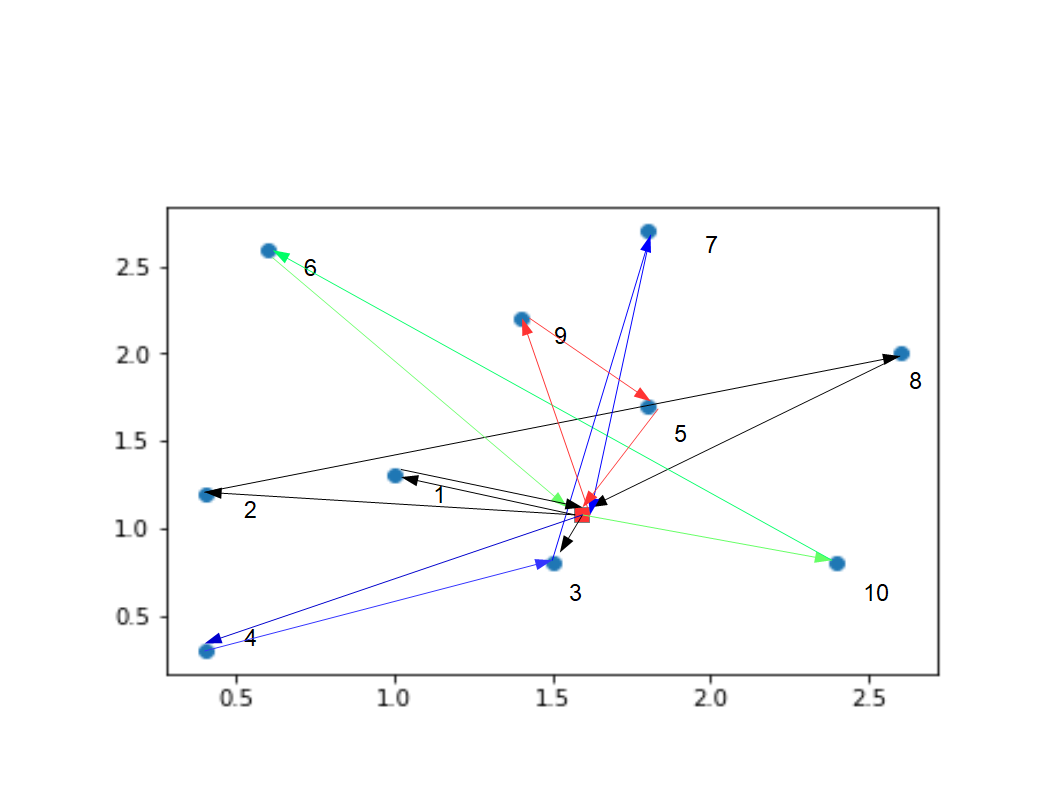
\includegraphics[width=150mm]{vrppp2.png}
    \caption{Mögliche, solide Lösung des VRP}  \label{Typen}
    {\footnotesize \textbf{blau:} Fahrzeug 1, \textbf{rot:} Fahrzeug 2, \textbf{schwarz:} Fahrzeug 3, \textbf{grün:} Fahrzeug 4, \textbf{orange:} Fahrzeug 5}
  \end{center}
\end{figure}

Es werden somit alle 10 Gene des Chromosoms bzw. alle 10 Kunden durch die Tourenplanung abgedeckt, ohne dass dabei eine Restriktion gebrochen wird.
Um nun in Erfahrung zu bringen, wie effizient das vorliegende Chromosom ist in Bezug auf die Kosten, die es verursacht, ist, wird im genetischen Algorithmus eine Evaluation durchgeführt, mit der die Fitnessfunktion berechnet wird. 
Nur anhand dieser Fitnessfunktion ist es dem genetischen Algorithmus möglich, effizient zu selektieren und sich iterativ weiterzuentwickeln.


\subsubsection{Evaluation des Chromosoms im genetischen Algorithmus}

Der Evaluationsprozess ist dafür zuständig, durch spezielle Methoden innerhalb des genetischen Algorithmus neuartige Chromosome innerhalb der Population zu bilden, sodass im Anschluss die Fitnessfunktion dieser berechnet werden kann und dadurch die Chromosome in der Population geordnet werden können, um somit die Selektion für die nächste Generation einzuleiten.
In dieser Evaluation werden zunächst die jeweiligen Routen der einzelnen Fahrzeuge auf deren Kosten untersucht, im Anschluss zusammengeführt, wobei diese Summe schließlich den Nenner der Fitnessfunktion bildet:

\begin{center}
max F(x) = $\frac{1}{totalCost}$
\end{center}

Kostenverursachende Faktoren sind hierbei lediglich die beiden Einheiten der Zeit- bzw. Distanz, welche beide als gleich kostenverursachend angesehen werden, sodass nur der Lieferweg sowie die Mietung eines neuen Roboters Kosten verursacht.

Das zuvor betrachtete Chromosom war das beste aus einer Anfangspopulation, die dadurch zustande gekommen ist, dass Chromosome zufällig zusammengewürfelt wurden.
Für jedes einzelne wurde im nächsten Schritt die Fitness berechnet, wobei das Chromosom [4, 3, 7, 9, 5, 2, 8, 6, 10, 1] mit dem Fitnesswert 0.0002537 am besten abschnitt und somit näher durchleuchtet wurde.
Nun besteht jedoch die Möglichkeit, dass dies bei weitem nicht das Chromosom ist, da es lediglich das beste Chromosom aus der zufällig generierten Anfangspopulation ist, die aus 100 Chromosomen besteht.
Um dies herauszufinden, wurde in dieser Arbeit ein genetischer Algorithmus angewandt, für den bereits die Vorarbeit in Form der Generierung der Anfangspopulation geschaffen wurde.

\subsubsection{Crossover und Mutation}

Im nächsten Schritt wendet dieser Algorithmus in der ersten Iteration einen Crossover an, wodurch zwei zufällig gewählte Chromosome ausgewählt werden und auf eine zuvor festgelegte Art und Weise miteinander verknüpft werden, sodass am Ende zwei neue Chromosome entstehen, die wiederum in der Population mitaufgenommen werden.
Bei diesem Crossover kann es sich um die verschiedensten Methoden handeln, die jedoch stets auf Zufallsprozessen basieren.
Der genetische Algorithmus, der in dieser Arbeit Anwendung fand, schnitt dabei eine bestimmte Sequenz aus dem Chromosom, bspw. [5, 2, 8] und addierte diese mit der kompletten Sequenz eines weiteren Chromosoms, sodass diese drei Gene dem zweiten, anderen Chromosom voran standen und in der Sequenz nun doppelt vorkamen. 
Die Doppelgänger, deren Pendant bereits schon einmal in der nun künstlich verlängerten Sequenz vorkamen, wurden gestrichen, sodass wiederum ein völlig neues Chromosom entstanden ist.

Dieser Vorgang wird für einen bestimmten Anteil der Chromosome vorgenommen, wobei dieser Anteil durch die vorher bestimmte Crossover-Wahrscheinlichkeit bestimmt wird. 
In dieser Arbeit konnten mit einer Crossover-Wahrscheinlichkeit i.H.v. 0.7 die besten Ergebnisse erzielt werden, sodass aus der Anfangspopulation von 100 Chromosomen ca. 70 Chromosome 35 Chromosompaare bildeten, die wiederum 70 neue Chromosome erschaffen haben, sodass im Anschluss der ersten Iteration eine neue Population mit insgesamt 170 Chromosomen entstanden ist. 
Aus diesen 170 Chromosomen werden nun abermals mit einem Zufallsprozess die 100 überdurchschnittlich besten Chromosome mit in den nächsten Iterationsschritt mitaufgenommen, wobei darauf geachtet wird, dass mindestens der beste aus den 170 Chromosomen mit in diesen Schritt genommen wird, um die beste Lösung nicht zu verlieren und ggf. nicht noch einmal zu erhalten, was ein herber Verlust wäre und nicht im Sinne einer Optimierung wäre.

Bevor dieser finale Schritt innerhalb einer Iteration allerdings in die Wege geleitet wird, wird ein kleiner Bruchteil der Chromosome (hier: 1\%) nochmals mutiert, um zu gewährleisten, dass die Konvergenz des Algorithmus nicht zu früh eintritt und dieser sich u.U. in einem lokalen Minimum befindet. 
Auch hierbei existieren diverse Mutationsprozesse, die auf Zufallsmechanismen beruhen, wobei in dieser Arbeit auf einen Prozess zurückgegriffen wurde, der wiederum eine Sequenz des Chromosoms [5, 2, 8] herausschneidet und dieses an gleicher Stelle spiegelverkehrt [8, 2, 5] wieder einsetzt.\\

Nachdem 100 Iterationen mit einer Crossover- bzw. Mutations-Wahrscheinlichkeit i.H.v. 0.7 bzw. 0.01 bei einer Populationsgröße von 80 durchgeführt wurden, ergibt sich ein Chromosom, dass eine Fitness von 0.00010454 erreicht wird, was auch nach mehreren Durchläufen unerreicht bleibt und somit einen äußerst guten Wert darstellen sollte.
Das Chromosom nimmt dabei folgende Form an: 

\begin{center}
[10, 8, 7, 9, 6, 4, 2, 1, 3, 5]
\end{center}

und verteilt sich dabei wie folgt auf die drei zur Verfügung stehenden Fahrzeuge: 


\begin{equation} \label{eq:test}
    \begin{aligned} 
         Fahrzeug 1&: 0 - 10 - 8 - 7 - 9 - 6 - 0 \\
        Fahrzeug 2&: 0 - 4 - 2 - 1 - 3 - 5 - 0\\
    \end{aligned}
\end{equation}


\begin{figure}[h!]
  \begin{center}
    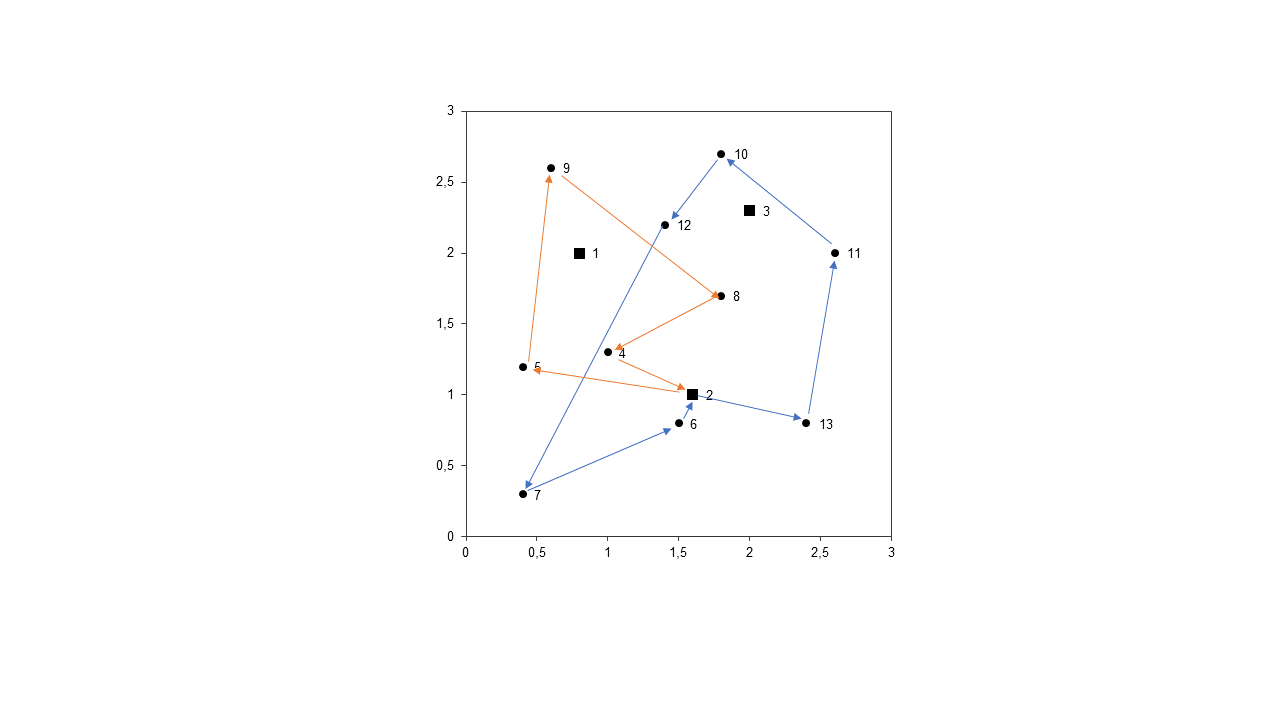
\includegraphics[width=150mm]{vrp22.png}
    \caption{Optimale Lösung des VRP}  \label{Typen}
	{\footnotesize \textbf{orange:} Fahrzeug 1, \textbf{grün:} Fahrzeug 2, \textbf{schwarz:} Fahrzeug 3}
  \end{center}
\end{figure}




\newpage


Nachdem das EVRP-TW erfolgreich mit einem genetischen Algorithmus analysiert und effizient gelöst werden konnte, wobei sich stets an die Angaben aus dem GAMS-Modell orientiert wurde, sowohl was die Informationen in der Instanz als auch die Parameter angeht, wird diese Herangehensweise im folgenden Kapitel mit der von Kleinschmidt (2017) verglichen.


\subsection{Implementierung des Algorithmus zur Lösung des FLP in das ERP-TW}


Nachdem die optimalen Standorte mit dem modifizierten Facility Location Problem herausgefunden werden konnten, werden diese einzeln für sich mit dem Vehicle Routing Problem mittels genetischen Algorithmus konfrontiert, so wie dies schon in Kapitel x vollzogen wurde.
Die Herausforderung dabei ist, dass es sich anstatt einer einzigen nun um mehrere Basisstationen handelt, deren Kunden so effizient wie möglich abgefahren werden sollen.
Die Kundenzuordnung wurde dabei bereits zuvor bei der Lösung des FLP ermittelt, sodass diese Information im nächsten Schritt dem genetischen Algorithmus übermittelt werden sollen, wodurch eine sequentielle Bearbeitung des Problems entsteht.

Die Zielfunktion orientiert sich dabei an der Zielfunktion in Kleinschmidts Modell, wobei auch hier die Mietkostenpauschale für alle neu eröffneten Basisstationen konstant sind. 
Öffnungs- bzw. Schließzeiten orientieren sich am GAMS-Modell und werden bereits in der Zielfunktion des FLP berücksichtigt.
Allerdings wird im genetischen Algorithmus nicht mit Zeitslots gearbeitet, so wie dies bei Kleinschmidt gehandhabt wurde.
Im genetischen Algorithmus entspricht hingegen eine Zeiteinheit genau einer Distanzeinheit und der Lieferroboter legt diese Distanzeinheit auch in genau einer Zeiteinheit zurück, sodass dies im Folgenden einer Modifikation bedarf, indem die Distanzeinheiten explizit durch die Geschwindigkeit geteilt wird, die dem Lieferroboter als Parameter gegeben wird.

Zu Vergleichszwecken wird dies dem Algorithmus bei Kleinschmidt insoweit angepasst, dass Angaben in Zeitslots mit dem Faktor 60 multipliziert werden, sodass im GA mit Zeiteinheiten in Minuten gerechnet wird. 
Auch wird dem Lieferroboter wie schon bei Kleinschmidt eine Durchschnittsgeschwindigkeit von 75m/min gegeben, sodass alle Distanzeinheiten, die bei der Berechnung von Ankunftszeiten verwendet werden, durch diese Geschwindigkeit geteilt werden (s. Gleichung (25)).
Die Entfernungen zwischen den Kunden bzw. Basisstationen werden in Metern angegeben.
Der Parameter $\alpha_{g,h,k}$, der den Wert 1 annimmt, wenn der Standort g vor dem Standort h auf der Route k angefahren wird, ist im genetischen Algorithmus nicht nötig, da die Routen durch die Chromosome genauestens definiert sind und lediglich abgefahren werden.

Somit fällt Restriktion (3) aus dem GAMS-Modell weg,  da der genetische Algorithmus bereits feste Touren durch seine Chromosome festlegt, sodass direkt ersichtlich wird, welcher Ort potentiell vor einem anderen Ort angefahren werden könnte.
So wird auch jeder Kunde nur einer Tour zugeordnet (Restriktion (2)), da jeder Kunde lediglich von einer Basisstation angefahren werden kann und von eben jener auch nur ein einziges Mal.

Aufgrund der festen Vorbestimmtheit der Touren durch das Chromosom und des Abfahrens eben jenes wird zudem sichergestellt, dass jeder Standort auch jeweils einmal angefahren und verlassen wird, sich nicht selbst anfährt, keine Kurzzyklen entstehen und ein Ort auch nur innerhalb einer Tour angefahren werden kann, wenn er sich auf eben jener befindet (Restriktion (4,5,6)).
Die Kapazität des Fahrzeugs in Gestalt von Compartements ist auch bereits im Algorithmus integriert und wird bei der Planung der Routen berücksichtigt.
Bei Betrachtung der einzelnen Basisstationen wird auch eine Variable zur Kapazitätsbeschränkung eben jener eingeführt, wobei diese sich wiederum an der Variable $Cap_{j}$ aus dem GAMS-Modell orientiert.

Um die Problematik auf ein elektrisches Problem umzumünzen, wurde bereits im genetischen Algorithmus eine Akkukomponente eingeführt, bei der lediglich bzgl. Zeit- und Distanzeinheiten angepasst werden.
Konnten die Zeitfenster im genetischen Algorithmus aus Kapitel x noch unter- bzw. überschritten werden, was mit erheblichen Kosten verbunden war, so ist dies in der Implementierung des FLP in den genetischen Algorithmus aus Vergleichszwecken nicht mehr gestattet. 
Da es jedoch sinnvoll sein könnte, diese Zeitfenster nicht immer einzuhalten und bewusste Verzögerungen mit einfließen zu lassen, werden diese Über- bzw. Unterschreitungen im nachfolgenden Kapitel diskutiert.
Das Modell, das nun durch den Algorithmus zur Lösung des FLP ergänzt wird, arbeitet somit ebenfalls mit Zeitbeschränkungen, so wie dies auch schon beim GAMS-Modell der Fall war, wobei sich an den Öffnungs- bzw. Schließungszeitpunkten der Zeitfenster der jeweiligen Kunden orientiert wird, die auch schon in diesem Modell verwendet wurden.

Binärvariablen, wie sie im GAMS bzw. im Algorithmus zur Lösung des FLP vorkommen, sind bei der Lösung des VRP durch den GA nicht vorgesehen.
Eine besondere Herausforderung bei der Implementierung besteht darin, dem genetischen Algorithmus die Kunden und ihre dazugehörigen Basisstationen, die durch die vorherige Standortbestimmung ermittelt wurden, zu übermitteln.
Dafür wird diese Information der Stationszuweisung direkt im Anschluss an die Lösung des FLP in die Instanz implementiert, die dann wiederum vom genetischen Algorithmus abgerufen wird.
Nur auf Basis dieser Information ist es dem GA möglich, eine gesonderte Betrachtung für jede einzelne Basisstation durchzuführen.
Eben jene Betrachtung wird durchgeführt, indem die Instanz in drei verschiedene Instanzen aufgeteilt wird, wobei jede Instanz für sich die Informationen über Kunden und Fahrzeuge enthält, die für die jeweilige Basisstation von Bedeutung sind.
Nur so kann der genetische Algorithmus explizit die Basisstationen gesondert untersuchen und deren optimale Touren vereinzelt planen. 
Nachdem der genetische Algorithmus die separate Instanz aufgenommen hat, baut er wiederum eine Anfangspopulation aus einer bestimmten Anzahl an Chromosomen, die wiederum exakt so viele Gene in sich beinhalten wie Kunden derjenigen Basisstation zugeordnet sind, deren Instanz untersucht wird.

Bei der Routenplanung wird dann das zufällig generierte Chromosom abgelaufen und die Gene solange einer Route zugeordnet, bis eines der Kriterien die Beschränkungen nicht eingehalten wird, wobei folgende Einschränkungen einzuhalten sind: 
Zum einen muss die Akkukapazität sowohl bzgl. seiner Laufzeit als auch seiner Reichweite vom Kunden, dessen Hinzunahme zur Route im aktuellen Schritt überprüft wird, zum Depot reichen. 
Ist dies nicht der Fall, bricht der Algorithmus an dieser Stelle ab und verweist den Kunden auf eine neue Tour.
Der Puffer, den der Akku dabei im GAMS-Modell sowohl hinsichtlich seiner Laufzeit als auch seiner Reichweite bekommen hat, wird im Algorithmus nicht extra erwähnt sondern direkt von der Akkulaufzeit bzw. -reichweite abgezogen, was lediglich der Übersichtlichkeit der Codierung geschuldet ist.

Auch die Ladekapazität des Fahrzeugs muss für diesen zusätzlichen Kunden ausreichen (Restriktion (7)), wobei sich diese dabei am Parameter $Comp$ aus dem GAMS-Modell orientiert, der die Compartements eines Fahrzeugs angibt, welche in der gleichen Einheit angegeben werden wie auch schon die Nachfrage der einzelnen Kunden.
Bereits im FLP wurde eine Restriktion eingeführt, sodass gewährleistet wird, dass alle Kunden auch ausreichend versorgt werden von den kapazitätsbeschränkten Basisstationen.
Zuletzt kann der Kunde auch nur dann mit in die aktuelle Tour aufgenommen werden, wenn bei der Ankunftszeit dass Zeitfenster eingehalten wird, dass dieser Kunde bei seiner Bestellung angegeben hat.
Dabei muss nicht nur die Fahrzeit berücksichtigt werden, die das Fahrzeug vom Kunden, bei dem es momentan anwesend ist, berücksichtigt werden, sondern auch die Service-Zeit, in der das Fahrzeug beim Kunden verweilt. 
So orientiert sich das Verfahren im Einzelnen am Verfahren, welches bereits in Kapitel x detailliert vorgestellt wurde.










\subsection{Diskussion der Ergebnisse}

Die im Kapitel x vorgestellte Herangehensweise stellt eine kombinierte Herangehensweise an die Problemstellung der Nutzung elektrisch betriebener Lieferroboter in der urbanen Logistik dar, wobei sich diese Herangehensweise aus der sequentiellen Bearbeitung des FLP und des ERP-TW zusammensetzt.
Das vorangegangene FLP wurde dabei mit Pythonversion 3.6.3 berechnet, welches sich einer Optimierungssuite bediente, die auf ein Branch-and-Bound-and-Price Verfahren zurückgriff, wobei der Solver SCIP für eine gemischt-ganzzahlige Modellformulierung exakt dieses Verfahren angewandt hatte (Quelle: scip.com).
Ziel des Algorithmus zur Lösung des FLP war es, dieses mit minimalen Kosten im Hinblick auf kostenverursachende Lieferwege effizient zu lösen.



Im Algorithmus zur Lösung des FLP verhält es sich bei der Deklarierung der Variablen ähnlich zu dem im GAMS-Modell, sodass auch in der Syntax von Python Variablen entweder als "binär" oder als "Integers" einzustufen sind, um der Optimierung keine Berechnungen zu verlangen, deren Bearbeitungszeit den Rahmen sprengen würden.

Die Ergebnisse, die daraufhin im genetischen Algorithmus zustande gekommen sind, wurden ebenfalls mithilfe des Analysetools Python in der Version 3.6.3 berechnet, da dies einer leichteren Implementierung der Ergebnisse aus dem FLP dienlich war.
Die Leistung des dabei zum Einsatz gekommenen Rechners (Windows 10, 64-Bit, Intel Core i5 8250U) ist bei 1.60GHz mit 4 Kernen und einem Arbeitsspeicher von 8GB einzustufen, sodass es vor diesem Hintergrund Sinn ergeben könnte, Abbruchkriterien in den Algorithmus mit aufzunehmen.
Wurde auf dieses noch im FLP verzichtet, so wurde beim genetischen Algorithmus ein Abbruchkriterium i.H.v. von 100 Iterationsschritten eingeführt.
Einschränkungen der Variablen im FLP wurden dabei nicht vorgenommen.

Der betrachtete Anwendungsfall bezieht sich wie bei bereits im Diskussionsteil des GAMS-Modell auf ein Stadtgebiet mit 13 fiktiven Orten, 3 für die Basisstationen und die restlichen 10 für die Kunden, wobei die Lage der Orte auf Abbildung x entnommen werden kann.
Auch entspricht die Entfernung zwischen den Orten der euklidischen Distanz zwischen den x- bzw. y-Koordinaten, die in der Instanz zur Verfügung gestellt werden.

Eine Ermittlung der Lösung kam bereits nach 1.27753 Sekunden zustande, wobei durch diese Gesamtkosten i.H.v. 825.1491 Einheiten aufkommen.
Durch das vorangegangene FLP wurden Basisstationen an den Orten 2 und 3 eröffnet, wovon allerdings insgesamt 7 Touren durch den genetischen Algorithmus als die optimale Tourenanzahl ermittelt wurden.
Veranschaulicht werden diese Routen in der folgenden Abbildung, wobei sogleich auffällt, dass die beste Lösung des metaheuristischen Verfahrens aus vielen Einzelteilen besteht.  



\begin{table}[h!]
    \vspace*{-3mm}
    \hspace*{2mm}
  \renewcommand{\arraystretch}{1,5}
  \caption{Lösungen der sequentiellen Herangehensweise
  }
  \begin{center}
 
    \begin{tabular}{|l|l|l|l|} \hline
    \textbf{Gesamtkosten (GE)} &\textbf{BS} &\textbf{Anzahl Touren}&\textbf{ Rechenzeit} (Sek)\\\hline
     825.1491 & 2;3 & 7 & 1.27753\\\hline   
	\end{tabular}
	  \end{center}
\end{table}


Die Routen der vier Touren der zweiten Basisstation sind folgende: 

\begin{equation} \label{eq:test}
    \begin{aligned} 
         Fahrzeug 1&: 0 - 10 - 8 - 7 - 9 - 6 - 0 \\
        Fahrzeug 2&: 0 - 4 - 2 - 1 - 3 - 5 - 0\\
    \end{aligned}
\end{equation}

Die Routen der drei Touren der dritten Basisstation sind folgende: 

\begin{equation} \label{eq:test}
    \begin{aligned} 
         Fahrzeug 1&: 0 - 10 - 8 - 7 - 9 - 6 - 0 \\
        Fahrzeug 2&: 0 - 4 - 2 - 1 - 3 - 5 - 0\\
    \end{aligned}
\end{equation}









Kritisch zu hinterfragen sind dabei die Einschränkungen, die dem in den vorangegangen Kapiteln vorgestellten Modell durch Kleinschmidt auferlegt wurden. 
So ist es zum für die Berechnungen zwar durchaus sinnvoll, jedem Kundenort lediglich eine Basisstation zuzuordnen, da dadurch die Komplexität der Problemstellung stark abnimmt. 
Allerdings ist es durchaus sinnvoll im Hinblick auf die Senkung der Gesamtkosten und auch in der Realität denkbar, dass ein Kunde von mehreren Basisstationen beliefert werden könnte, sodass sich dieser Idee in den Erweiterungen des Modells im anschließenden Kapitel gewidmet wird.
Zusätzlich zu der Erweiterung des Modells durch das Zulassen der Belieferung von Kunden durch mehrere Basisstationen erscheint eine weitere Zulassung sinnvoll: die Nichteinhaltung der Zeitfenster mit sich auf die Kostenfunktion negativ auswirkenden Kosten.






\newpage

\section{Erweiterungen}

\subsection{Zulassen von mehreren Belieferungen je Kundenort}

Aufgrund der stark eingeschränkten Kapazität des Fahrzeugs muss eine Tour häufig bereits nach wenigen Kunden abgebrochen werden, sodass es eine sinnvolle Erweiterung des Modells wäre, wenn jeder Kunde zusätzlich von weiteren Robotern, die sich auf anderen Touren befinden, beliefert werden könnte.
Dabei muss bereits in den Algorithmus zur Lösung des dem EVRP vorangegangenen  FLP eingegriffen werden, wobei eine Restriktionen eliminiert wird, um so zu gewährleisten, dass bereits im FLP jedem Kunden mehr als eine Basisstation zugeordnet werden kann.



\subsection{Belieferungen der Kundenorte außerhalb des Zeitfensters}

Da das Niveau des Kundenservices zu den wesentlichen Einflussgrößen hinsichtlich Kosten gehört, sollte es eigentlich außer Frage stehen, dass der Kunde auch in seinem Zeitfenster beliefert wird.
Sollte es sich allerdings nur um kurze Verspätungs- bzw. Wartezeiten des Fahrzeugs beim Kunden handeln, sodass dieser dafür im Umkehrschluss allerdings mit auf eine bereits bestehende Tour genommen werden kann, so könnte es durchaus sinnvoll sein, dieses Zeitfenster mit vorheriger Benachrichtigung und einem Einverständnis des Kunden zu über- bzw. unterschreiten.
Diese Warte- bzw. Verzögerungszeiten würden sich dann wiederum auch negativ auf die Kosten einer Tour auswirken, wobei diese Kosten dann eher immaterieller Natur wären in Form von Imageschäden. 
Abgewogen sollte in diesem Zusammenhang auch die Frage, wie hoch diese Kosten in Relation zu anderen Kosten sein sollten.

Es würde so allerdings gelingen, den Kunden 4, der zur Basisstation 2 zugehörig ist, mit auf die erste Tour zu nehmen und so eine Neuinitialisierung eines Lieferroboters speziell für diesen Kunden aus dem Weg zu gehen, wie folgende Abbildung zeigt: 




\subsection{Diskussion der erweiterten Modelle}




\newpage
\section{Limitationen und Handlungsempfehlungen}


Im Folgenden wird zunächst untersucht, welchen Limitationen bei der Bearbeitung der Problemstellung gegenübergetreten werden musste. 
Durch die sequentielle Bearbeitung der Problemstellung war es teilweise äußerst mühselig, die Informationen, die durch die Lösung des FLP zustande gekommen sind, in das anschließende Verfahren zur Lösung des VRP zu übermitteln, sodass sich im Nachhinein für eine andere, eher simultane Bearbeitung entschlossen werden würde.

Eine Schwierigkeit bei der Implementierung des genetischen Algorithmus in Python stellte vor allem die Angelegenheit dar, dem Lieferroboter seine genaue Startzeit am Depot mitzuteilen. 
So startete dieser, wenn das Depot eröffnete in der Hoffnung, den ersten Kunden im Chromosom auch in seinem Zeitfenster zu erreichen. 
Gelang dies nicht, so wurde der Kunde direkt einer neuen Tour mit einem neuen Lieferroboter zugewiesen. 
Falls dies geschieht, so startet der neue Lieferroboter exakt zu dem Zeitpunkt an der Basisstation, sodass er genau pünktlich zum Beginn des Lieferfensters am Standort des ihm neu zugewiesenen Kunden ankommt.
Dadurch kommt es vor, dass der Lieferrobotern bei manchen Kunden an späterer Stelle im Chromosom zu früh ankommt, obwohl es im Bereich des Möglichen gewesen wäre, bei einer späteren Ankunft beim ersten Kunden im Chromosom diesen späteren Kunden noch mitzunehmen.
Bspw. geschieht dies im GAMS-Modell, wie der Abbildung 3 zu entnehmen ist. 
Hier wird der erste Kunde einer Tour, Kunde 6, erst sehr spät angefahren, sodass es möglich ist, auch den Kunden 4 noch mit auf die Tour zu nehmen, dessen Zeitfenster sich erst um 12 öffnet. 
Im genetischen Algorithmus hingegen wäre der Kunde 6 bereits zum frühesten Zeitpunkt, hier um 8 Uhr, angefahren worden, sodass der Kunde 4 nicht mehr mit auf die Tour mitgenommen wird, worunter die Effizienz der Tour leidet.
Der erste Lieferroboter mit der leeren Tour wurde im Anschluss an die Touroptimierung zwar gelöscht, sodass keinerlei Kosten in Form von einer Mietkostenpauschale entstanden ist, jedoch wäre eine direktere Anweisung seiner Startzeit nicht nur wünschenswert sondern vor allem auch unter Umständen optimierend gewesen.


Anschließend an die eben beschriebenen Limitationen werden im Folgenden Handlungsempfehlungen dargelegt, durch die potentielle Verbesserungen des Modells in die Wege geleitet werden könnten.

Da es wie in der Diskussion zum GAMS-Modell bereits angesprochen sinnvoll erschien, dass Tourenproblem nicht ebenfalls simultan zum Standortproblem ablaufen zu lassen, da letzteres einer gewissen Schnelllebigkeit ausgesetzt ist aufgrund der täglich variierenden Kundenstandorte.
Macht man nun das Standortproblem von der Tourenplanung abhängig, so wie dies im GAMS-Modell geschehen ist, so könnte eine optimale Lösung am nächsten Tag bereits wieder suboptimal bzw. schlecht sein.
Um dieser Angelegenheit etwas entgegenzusetzen, wäre es in einem fiktiven Fall möglich, dass man die optimalen Standorte nicht aus einer Menge an bereits geografisch feststehenden Standorten wählen muss, sondern eine gesamte Menge an potentiellen Kunden durch Clustermethoden zunächst zu clustern und diesen im gleichen Zuge ein Zentrum zuweisen würde, welches dann die Basisstation für die zu diesem Cluster zugewiesenen Kunden bildet.
Die Kunden könnten dabei eine gewisse Wahrscheinlichkeit zugewiesen bekommen, welche wiederum durch zweidimensionale Wahrscheinlichkeitsverteilungen wie einer Verteilung in Abhängigkeit einer Kernfunktion zustande kommen könnten, welche das Clusterverfahren zusätzlich gewichten könnte.

So würde durch den bspw. durch einen k-Means-Algorithmus aus einer Menge von Datenpunkten eine vorher festgelegte Anzahl von k Gruppen gebildet. 
Mithilfe eines 'K-means Algorithmus' wird anschließend für jede Gruppe k ein sogenanntes Clusterzentrum z gebildet.
Ziel ist es dabei das Zentrum so zu positionieren, dass die Summe der quadrierten Abweichungen aller Datenpunkte minimal ist (Vgl. Kanungo et.al S.881).
So würde auf das LRP bezogen dann also ein Depot gesucht werden, welches eine möglichst minimale Entfernung zu den Nachfrageorten (Kunden) besitzt.
Der Begriff 'K-means' wurde 1967 erstmals vom Mathematiker J.MacQueen verwendet (Vgl. J.MacQueen S.281-297).
%Der bekannteste K-means Algorithmus wurde jedoch schon 1957 von S.Lloyd publiziert, der sogenannte Lloyd-Algorithmus. Um den Algorithmus zu initialisieren werden zunächst z zufällige Mittelwerte (Clusterzentren) aus dem Datensatz gebildet.
%Anschließend wird jeder Datenpunkt einem Cluster zugeordnet, wobei die Zuordnung durch Varianzminimierung (d.h die geringste Entfernung zum Mittelwert) erfolgt. 
%
%Im nächsten Schritt folgt nun die Neuberechnung des Clusterzentrums anhand des Erwartungswertes.
%Nun werden die Datenpunkte wieder anhand der geringsten Entfernung zu einem Zentrum neu verteilt, in dem die Varianz aller Datenpunkte neu berechnet wird.
%Es handelt sich hierbei um eine iteratives Verfahren. 
%Der Algorithmus stoppt erst, wenn sich die Clusterzentren und die Zuordnung der Datenpunkte nicht mehr verändern (Vgl. Kanungo S.882).
%
%Der K-means Algorithmus von Lloyd ist ein anerkannter Algorithmus, jedoch weist er einige Probleme auf. 
%Durch die zufällige Auswahl von Startpunkten bei der Initialisierung ist es oftmals der Fall, dass die vorliegende Lösung nicht optimal ist. 
%Man müsste den Algorithmus mit verschiedenen Startpunkten mehrmals hintereinander laufen lassen um zu sehen welche Lösung optimal ist, was einen hohen Zeitaufwand mit sich bringen würde.
%Des Weiteren ist das K-means Clustering anfällig für Ausreißer (bei großen Entfernungen), die die Positionierung des Clusterzenrums stark verfälschen können. 
%Die Bestimmung der Anzahl der Clusterzentren z ist ebenfalls von Bedeutung. 
%Wird z zu klein gewählt, kann es zu hohen Distanzen zwischen Zentrum und den Datenpunkten kommen.\\

Der 'k-means-Algorithmus' wäre für die Zwecke in dieser Arbeit eine attraktive Lösung, da zum einen eine beliebige Anzahl an Depots optimal und somit kostenminimierend gefunden werden könnten.
Zum anderen wären die Kunden stets optimal zugeteilt, sodass ein hohes Maß an Flexibilität durch diesen Algorithmus entsteht, falls ein neuer Kunde hinzukommen oder abspringen sollte.
Allerdings besteht das Problem, dass zum einen in der Realität die Standorte der möglichen Basisstationen meistens vorgegeben sind.
Des Weiteren werden aus diesen vorgegebenen Standorten meist nur eine begrenzte Anzahl an Basisstationen ausgewählt, wobei diese Anzahl im Gegensatz zum k-Means-Algorithmus zuvor nicht feststeht. 
So ist es zusätzlich in der realen Welt nicht immer möglich, die vom k-Means-Algorithmus gefundenen Standorte mit Basisstationen zu bebauen, da dort eventuell die Bedingungen nicht gegeben sind.
Beispielsweise nimmt der Algorithmus keine Rücksicht auf geografische Besonderheiten wie Bergland, Gewässer oder sonstiges, unbebaubares Gelände.

Weitere Handlungsempfehlungen wären zudem, verstärkt auf Sensitivitätsanalysen zu setzen. 
Es könnten außerdem im Bereich der Erweiterungen noch auf die Konstellation eingegangen werden, dass ein Roboter nach einem Batterietausch wieder einsatzbereit wäre und zu einer nächsten Tour aufbrechen könnte.




\newpage
\section{Diskussion}

In diesem Teil der Arbeit werden die wichtigsten Aspekte sowie Ergebnisse der beiden untersuchten Modelle nochmals hervorgehoben und miteinander verglichen.

Zunächst ist es auffällig, dass die sequentielle Bearbeitung der Problemstellung mit deutlich schnelleren Bearbeitungszeiten einhergeht.
Obwohl sie durch einen deutlich schwächeren Prozessor (1.6GHz statt 2.5GHz) ausgeführt wurden, entsprachen die Bearbeitungszeiten der zweiten Herangehensweise nur einem Bruchteil derjenigen, die das GAMS-Modell mit einer nichtlinearen Modellkonstellation benötigte und kam dabei nur auf marginal schlechtere Ergebnisse.
Auch bei Umformulierung der Parameter und der damit erzeugten Linearisierung des Modells war das GAMS-Modell noch doppelt so langsam wie das sequentielle Modell.

Bei starker Ähnlichkeit der Ergebnisse könnte man demnach berechtigterweise zu dem Schluss kommen, dass es sinnvoller wäre, im Hinblick auf die Bearbeitungszeit anstatt des GAMS-Modells einen Algorithmus zu verwenden, der sich nur zu einem Teil auf einen optimierenden Solver stützt, einen anderen Teil jedoch in ein metaheuristisches Verfahren durch die Untersuchung des EVRP-TW mit einem genetischen Algorithmus ausgegliedert hat.
Bei näher Betrachtung der Ergebnisse im Detail war jedoch der Grund hierfür schnell auszumachen: das sequentielle Modell optimierte nicht die Startzeitpunkte, in der ein Lieferroboter die Basisstation verlässt und sich auf die Reise zum ersten Kunden der ihm zugewiesenen Tour macht, sodass der erste Kunde einer Tour stets zum frühesten Zeitpunkt angetroffen wird. 
Dies stellte insofern einen Nachteil dar, da bei bewusster Verzögerung des Starts eines Lieferroboters Kunden unter Umständen noch mit auf die Tour aufgenommen werden könnten, sodass hier an Effizienz eingebüßt wurde, welche sich auch in den unterschiedlichen Gesamtkosten direkt bemerkbar machten.
Die Bearbeitungszeit der hier vorliegenden Arbeit war leider zu kurz, um dem genetischen Algorithmus, der \textit{from scratch} (engl.: 'fast aus dem Nichts') erschaffen wurde, diese zusätzliche Eigenschaft einzuimpfen, sodass hier ein großer Raum für weitere Nachforschungen geschaffen wurde.
Diese Problematik des GA schlägt sich dann dementsprechend direkt auf die Bearbeitungszeit nieder, sodass an dieser Stelle von einem nicht-fairen Vergleich der beiden Bearbeitungszeiten gesprochen werden muss.

Aufgrund dieser Umstände ist es in den Lösungen des sequentiellen Modells dazu gekommen, dass es zu viel mehr Touren kam als im simultanen GAMS-Modell (7 statt 4), sodass ein Ziel, nämlich der Vermeidung von zu vielen Touren, im zweiten Modell deutlich verfehlt wurde.
Auffällig war, dass der dem EVRP vorangegangene Algorithmus zur Lösung des FLP die gleichen Ergebnisse hinsichtlich der optimalen Standpunkte der Basisstationen hervorbrachte, wie dies auch schon im simultanen GAMS-Modell geschah. 
Da die Lösungen, die durch den GA zustande gekommen sind, sehr zerstückelt und für die Praxis nahezu unbrauchbar sind, legt dies nur die Vermutung nahe, dass die simultane Herangehensweise die zwar etwas langsamere, aber doch effizientere Lösung für den operativen Einsatz zu sein scheint, wie dies auch schon an den geringeren Kosten deutlich wird.	









\newpage
\section{Schlussbemerkungen}



In der vorliegenden Arbeit wurde sich auf die Entwicklung eines Entscheidungsmodells zur Bestimmung optimaler Standorte von Basisstationen sowie Touren von Lieferrobotern innerhalb einer urbanen Umgebung fokussiert vor dem Hintergrund, dass jene Umgebung bis heute stetig am Wachsen ist und ihre Nachfrage in wirtschaftlicher Hinsicht befriedigt werden muss.
Speziell wurde dabei demnach auf die "letzte Meile" eingegangen, also die letzte Hürde, die bei einer Lieferung in Betracht gezogen werden muss, bevor der Kunde seine Ware erhält.

Es wurde versucht, dieser Problemstellung auf zweierlei Arten entgegenzutreten: einer optimierenden Variante, in der das Standort- sowie das Tourenproblem simultan mittels eines GAMS-Modells gelöst wurde und einer sequentiellen Variante, die das Tourenproblem mittels einer metaheuristischen Herangehensweise versucht hat zu lösen vor dem Hintergrund, bei allzu großen Datenmengen auf ausgiebige Rechenoperationen zu verzichten, um das Modell für die Praxis attraktiv zu gestalten.
Diese beiden Herangehensweisen boten sich gerade deshalb an, da sie in ihren Gestaltungen sehr flexibel sind, was für die Ausführungen solch neuartiger Konzepte, wie es Belieferungen mittels Roboter darstellen, unabdingbar war.











%%%%%%%%%%%%%%%%%%%%%%%%%%%%%%%%%%%%%%%%%%%%%%%%%%%%%%



\newpage
\bibliographystyle{Prod_Seminar}    %legt die zu verwendende BIBTEX-Stildatei fest
\bibliography{Literatur}    %an der Stelle zu verwenden, an der das Literaturverzeichnis gesetzt werden soll;
                            %Literatur ist der Dateiname der BIB-Datei mit den Literatur-Informationen

\newpage

\begin{appendix}
\section{aussagekräftige Überschrift für Inhalt des Anhangs}

\end{appendix}
%%%%%%%%%%%%%%%%%%%%%%%%%%%%%%%%%%%%%%%%%%%%%%%%%%%%%%
%
%   ENDE DES DOKUMENTS
%
%%%%%%%%%%%%%%%%%%%%%%%%%%%%%%%%%%%%%%%%%%%%%%%%%%%%%%

\end{document}
